% El comando "\chp" es como el "\chapter" pero mete "Chapter" en vez de "Capitulo"
\chp{9}{Conclusions and future work}
\noindent

% addtocounter: necesario para tener el mismo número de \section que el de español ==> -2 porque hay 2 secciones en el capitulo 9 - igual para las imágenes
\addtocounter{section}{-2}
\addtocounter{figure}{-1}

\section{Conclusions}
In this project we have developed an application that helps to manage the diet of an athlete, being able to choose a diet among those created by other users. 

Athletes can create diets that can later be followed by other users. In addition, athletes have the possibility to consult the detailed information of each of the foods that they should consume during the diet. At the same time, explanatory documents can be uploaded so that the athlete who follows the diet knows the purpose of each food within the diet, being able to provide more information to the user.

The current diet can be evaluated so that other athletes have references of it, being able, in turn, to comment on the diet followed.

% Despite the fact that the members had not previously worked with Android, nor had they developed similar applications for mobile devices, it is considered that the service developed provides the application users with the value that had been established at the beginning of the project, fulfilling the objectives set at the beginning.

In the following link you can view and download, from the GitHub repository, the code of the project as well as the executable application: \url{https://github.com/csegundo/Diet-Now}.

\section{Future work}
% The following is a description of a series of implementations that could be added to the application in order to improve the user's experience while using it.
The following are a number of ideas for future work that could be added to the application in order to improve the user's experience while using the application.

\begin{itemize}
    % \item \textbf{Dark mode:} the application is currently implemented with the clear theme, which is configured by default in many applications. There are several motivations that may lead us to implement this improvement, highlighting mainly the following.
    % \begin{enumerate}
    %     \item Visual comfort: setting a dark background in the application, such as black, gray or blue, reduces eye strain and prevents eye strain and fatigue. It also allows them to adapt more easily to dimly lit spaces.
    %     \item Battery saving: Battery saving: On most mobile devices, dark mode can help reduce battery life by 14\% to 60\%, depending on screen brightness.
    % \end{enumerate}
    
    \item \textbf{Bottom navigation bar:} the main objective of this implementation is to improve the user experience, allowing an easier and more intuitive navigation between the different views by adding a menu with a series of icons at the bottom of the screen.% In Figure \ref{fig:app_bottom_bars_en} a \textit{mockup} of this menu is shown in two different views of the application.
    % \begin{figure}[H]
    %     \centering
    %     \subfigure[View of the current diet]{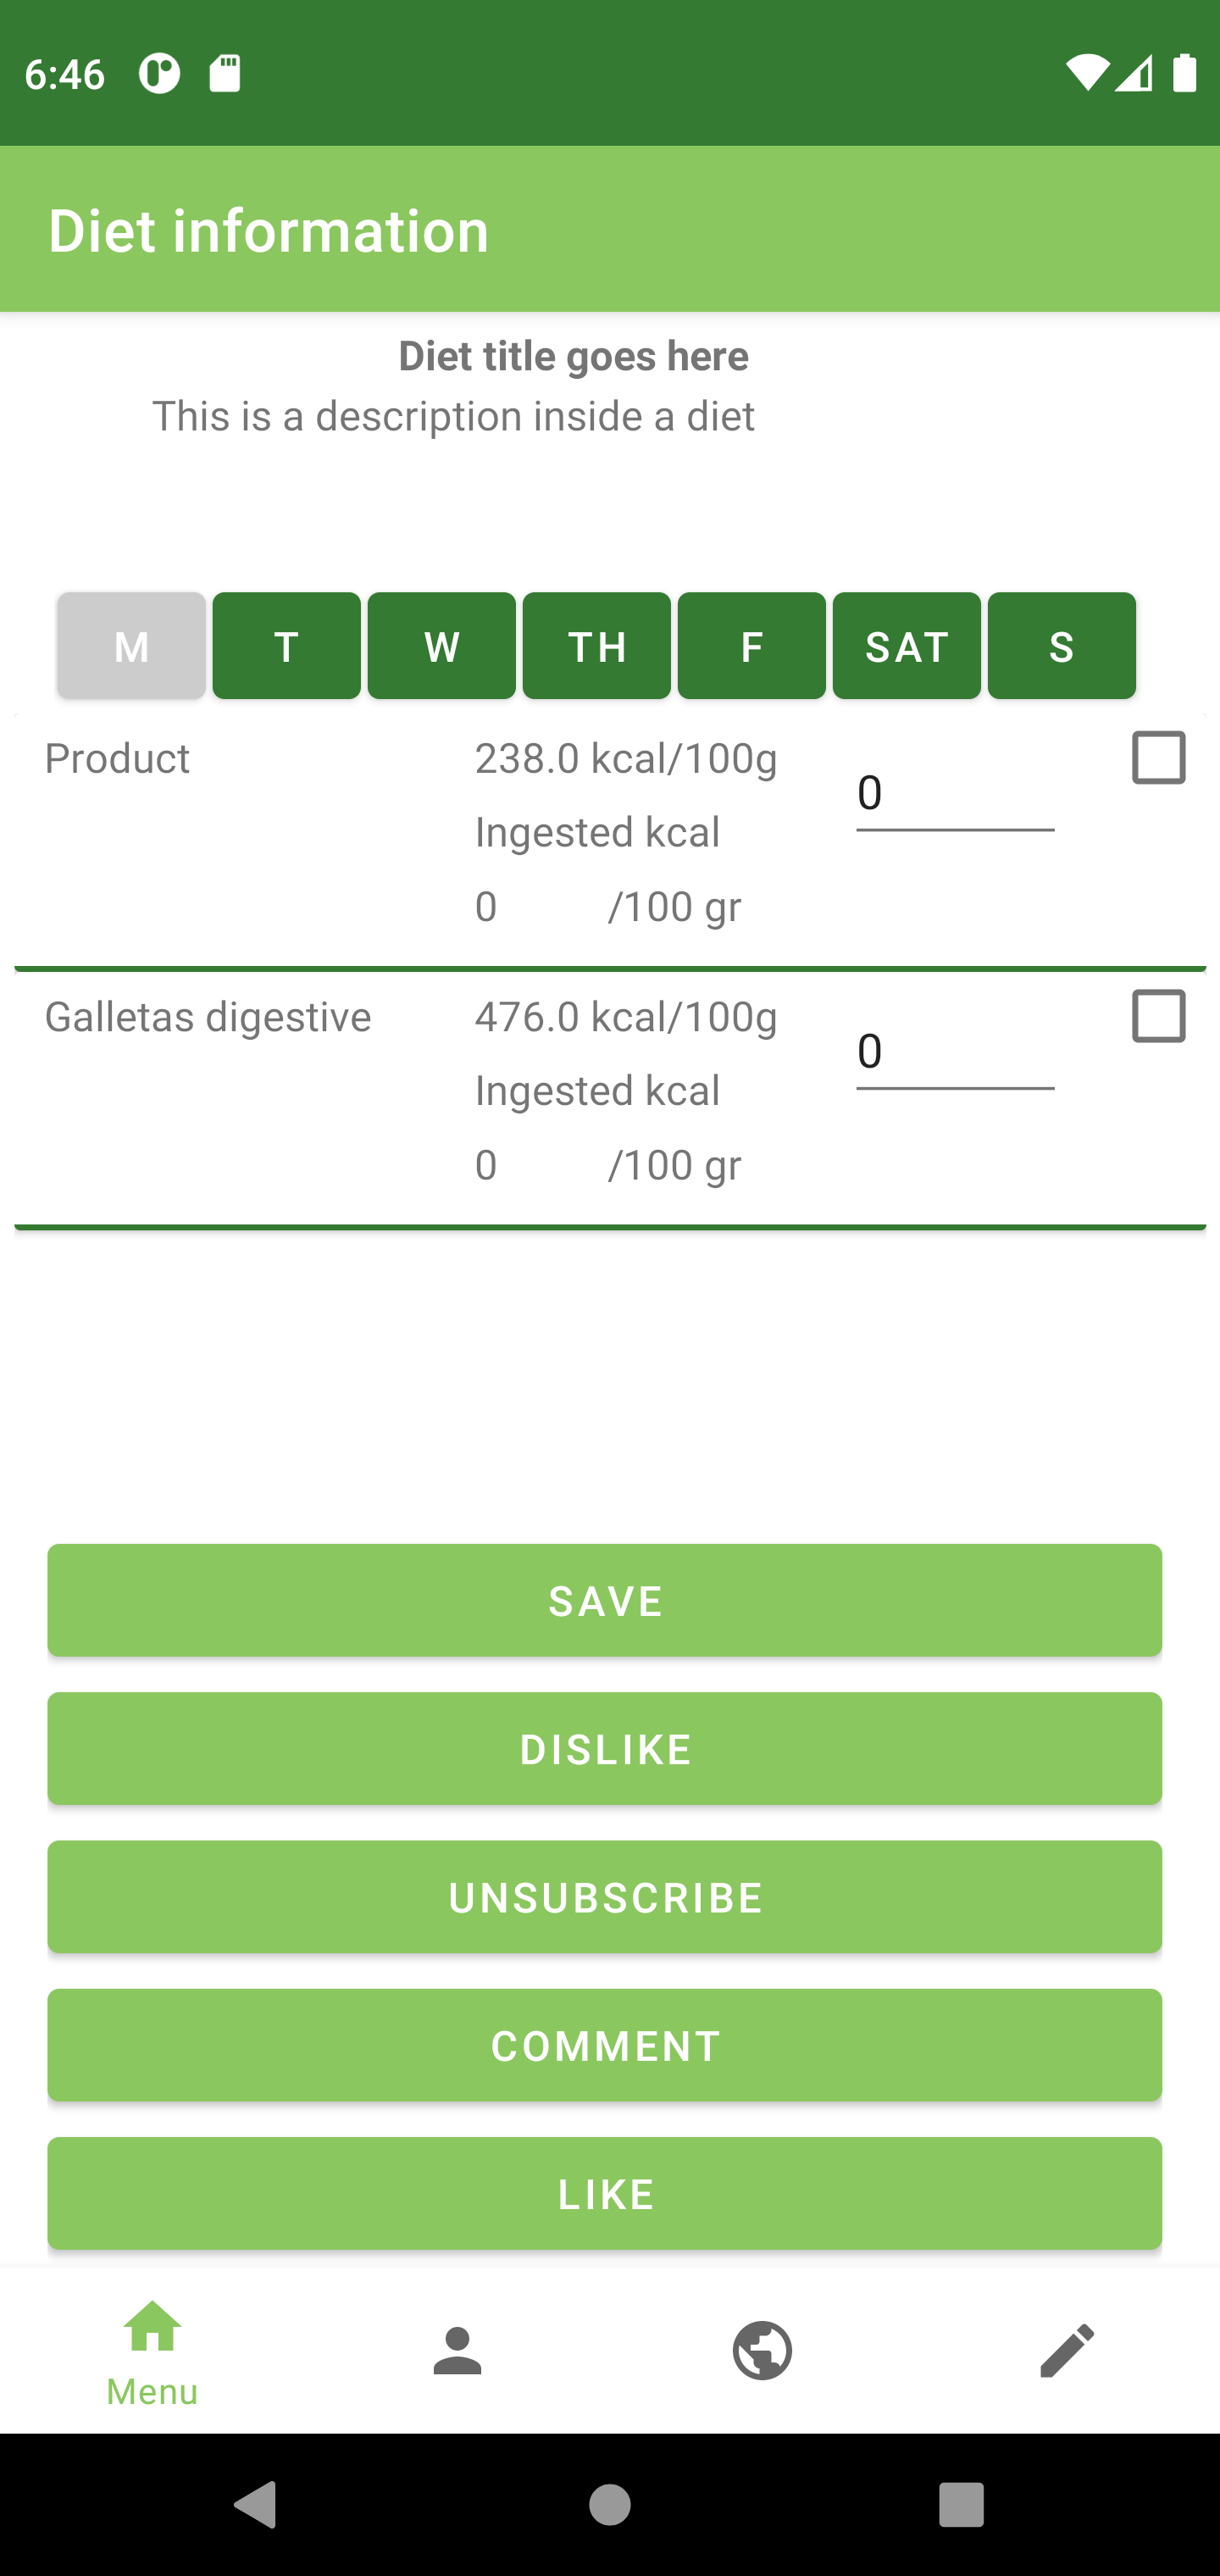
\includegraphics[width=0.45\textwidth]{Images/Capitulo9/bottomBar1_en.png}}
    %     \subfigure[Athlete profile view]{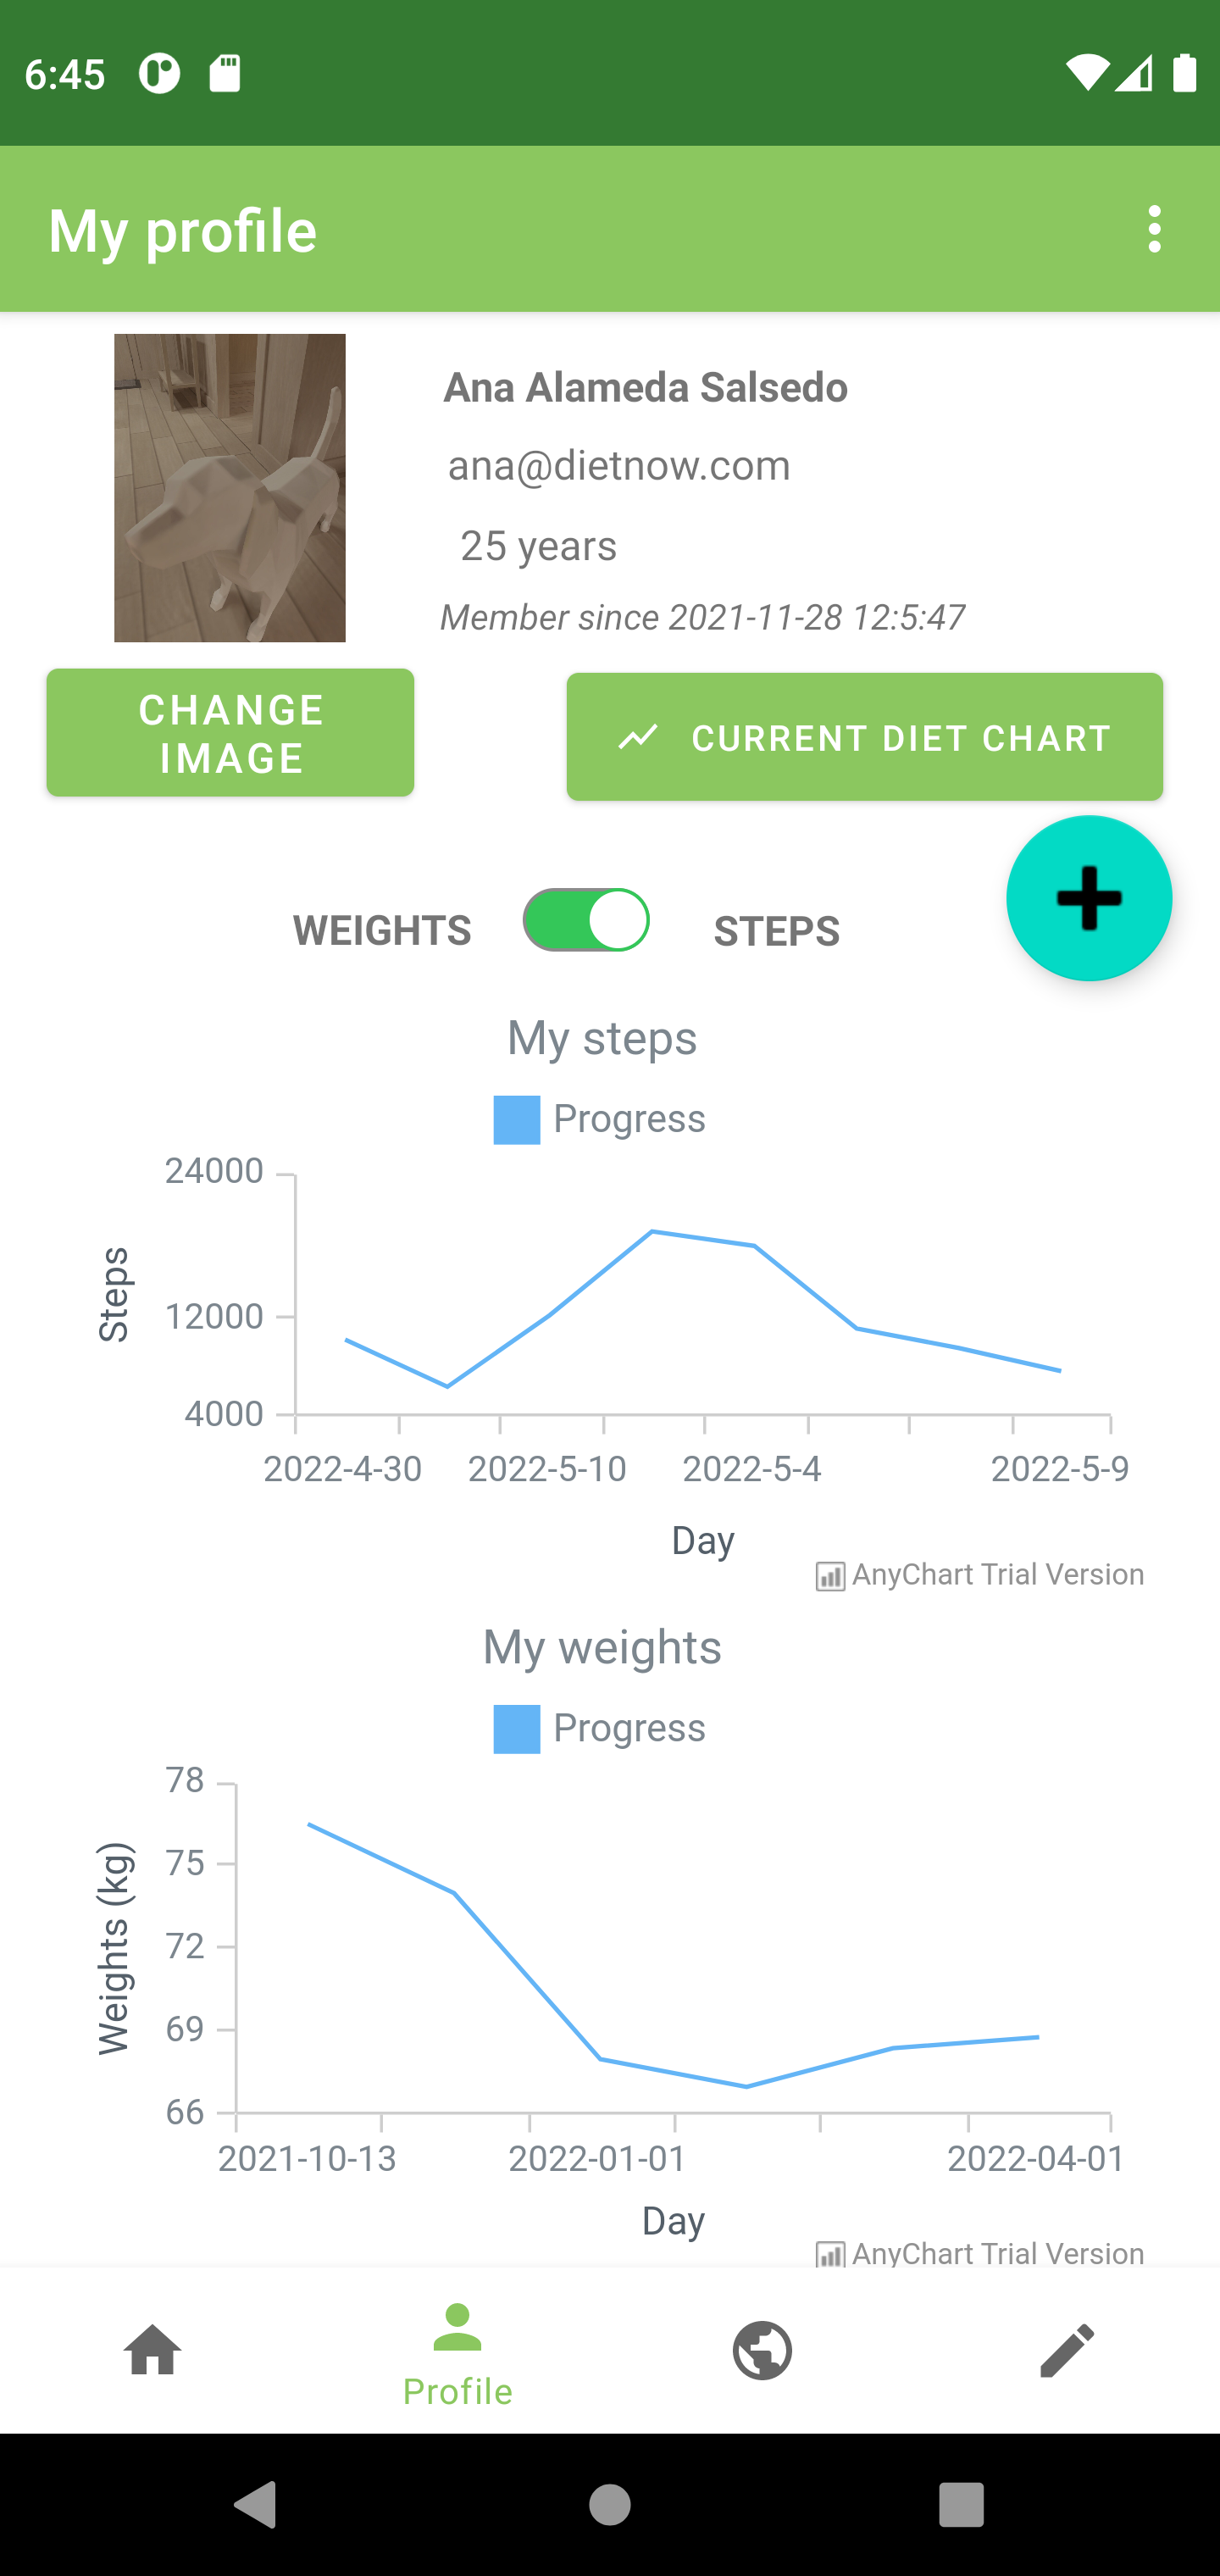
\includegraphics[width=0.45\textwidth]{Images/Capitulo9/bottomBar2_en.png}}
    %     \caption{\textit{Mockups} of the bottom menu in different views}
    %     \label{fig:app_bottom_bars_en}
    % \end{figure}
    
    % \item \textbf{Deploy the servers of \textit{Node.js} and \textit{Spring}:} to enable the application to reach all audiences, it could be possible to deploy both the \textit{Node.js} (which is responsible for calling the API of \textit{OpenFoodFacts}) as the server of \textit{Spring} (in charge of changing the fields of the \textit{Firebase Authentication} module explained above in the section \ref{google_firebase_tools}). One option would be to deploy these servers on \textbf{\textit{Heroku}}, a platform as a service (\textit{PaaS}) that would allow us to make calls to these APIs from any device since they are in the cloud and not locally.
    
    \item \textbf{Signing in with a Google or Facebook account:} to improve the usability of the application, this new functionality of logging in with a Google or Facebook account could be implemented. In addition to the benefit already mentioned, it could considerably increase the number of users in the application due to the fact that most Facebook users use a mobile device, as shown in Fig. \ref{fig:fb_users}.
    \begin{figure}[H]
        \centering
        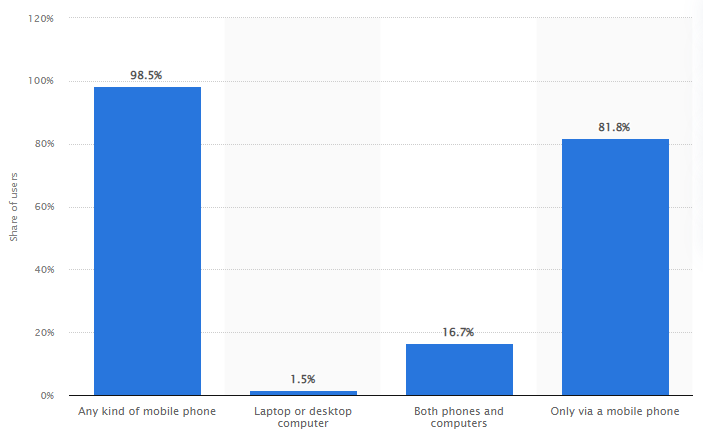
\includegraphics[width=\textwidth]{Images/Capitulo9/fbUsers.png}
        \caption{Devices used to log in to Facebook in January 2022 \cite{mobile_max_users}}
        \label{fig:fb_users}
    \end{figure}
    % https://www.statista.com/statistics/377808/distribution-of-facebook-users-by-device/
    
    \item \textbf{Reset password:} currently the application does not have a password recovery system in case the user does not remember the password. This implementation would make it easier for the user to regain access to their account when they forget their password by adding a new button on the login screen that sends an email to the user's email so that the user can reset the password from a link.
    
    \item \textbf{Adding foods in food groups:} give the athlete the possibility to add food to a diet in each of the five meals that are eaten throughout the day. When a food is to be added to a diet, the user specifies whether that food belongs to breakfast, lunch, afternoon snack...
    
    \item \textbf{Share diets:} allow users who use the application the possibility of sharing through other social or messaging networks all different diets they inserted into the application.
    
    \item \textbf{Connection with smart watches:} offer the possibility for the user to connect a wristband or smartwatch to the application. Through this connection, data such as the number of steps walked during the day can be collected and automatically entered into the user's account to be displayed on the step graph.
    
    \item \textbf{Connect diet management with Alexa or Google assistant:} allow users who create a diet the possibility of doing so by voice commands. This tool could also be used to generate a purchase through the Alexa or Google assistant with the stored products of a diet.
\end{itemize}